% Template for IGARSS-2020 paper; to be used with:
%          spconf.sty  - LaTeX style file, and
%          IEEEbib.bst - IEEE bibliography style file.
% --------------------------------------------------------------------------
\documentclass{article}
\usepackage{spconf,amsmath,epsfig}
\usepackage{subcaption}
\usepackage{multirow}
% Example definitions.
% --------------------
\def\x{{\mathbf x}}
\def\L{{\cal L}}

% Title.
% ------
\title{USING THE GAF TRANSFORM AND MODIS TIME-SERIES TO PERFORM LANDCOVER CLASSIFICATION AND CHANGE DETECTION}
%
% Single address.
% ---------------
\name{T.L. Grobler$^{\dagger}$, W. Kleynhans$^{\star}$ and B.P. Salmon$^{\ddagger}$}
\address{$\dagger$Dept of Mathematical Sciences, Computer Science Division, Stellenbosch University,\\ Private Bag X1, 7602 Matieland, South Africa\\
$\star$Department of Electrical, Electronic and Computer Engineering University of Pretoria,\\
Pretoria 0002, South Africa\\
${\ddagger}$School of Engineering, University of Tasmania,
Hobart, TAS 7001, Australia}
%
% For example:
% ------------
%\address{School\\
%	Department\\
%	Address}
%
% Two addresses (uncomment and modify for two-address case).
% ----------------------------------------------------------
%\twoauthors
%  {A. Author-one, B. Author-two\sthanks{Thanks to XYZ agency for funding.}}
%	{School A-B\\
%	Department A-B\\
%	Address A-B}
%  {C. Author-three, D. Author-four\sthanks{The fourth author performed the work
%	while at ...}}
%	{School C-D\\
%	Department C-D\\
%	Address C-D}
%
\begin{document}
%\ninept
%
\maketitle
%
\begin{abstract}
The Gramien Angular Field (GMF) transform encodes time-series into images so that image based classification approaches can be exploited to perform time-series classification. Settlement expansion is one of the most pervasive forms of landcover change in sub-saharan Africa. In this paper, we show that the GAF transform outperforms the conventional techniques we compared against when it is employed in conjunction with Moderate Resolution Imaging Spectroradiometer (MODIS) time-series to detect settlement expansion in the Gauteng province of South Africa.   
\end{abstract}
%
\begin{keywords}
Moderate Resolution Imaging Spetroradiometer, Gramian Angular Fields, landcover classification and change detection, settlement expansion
\end{keywords}
%
\section{Introduction}
\label{sec:intro}
The field of computer vision has changed dramatically over the last few years due to the success of Convolutional Neural Networks (CNNs) and deep learning \cite{goodfellow2016}.  Recently, it was proposed to encode time-series as images so that the capability of CNNs to perform image classification could also be applied to the problem of time-series classification \cite{wang2015}. One possible time-series encoding scheme is the Gramian Angular Field (GAF) transform. GAF images are formed using polar coordinates and ultimately take the form of a Gramian matrix, whose entries are the trigonometric sum of observations recorded at different time indices.  Dias et al. used the GAF transform (and other transforms), Moderate Resolution Imaging Spectroradiometer (MODIS) time-series and existing CNN models to successfully detect eucalyptus plantations \cite{dias2019}. Their CNN based solution outperformed the conventional approaches they compared against. In this paper we will investigate whether MODIS time-series and the GAF transform can be utilized for detecting settlement expansion. Settlement expansion is one of the most pervasive forms of landcover change in sub-saharan Africa. It is, therefore, of the utmost importance to find strategies and algorithms that will allow us to effectively monitor the growth of settlements in Africa. In this paper, however, we will restrict ourselves to a case study in the Gauteng province of South Africa. In addition to investigating another use case than Dias et al. we also extend their work in the following ways:
\begin{itemize}
 \item We do not restrict ourselves to only investigating the problem of land cover classification, we also investigate whether the GAF transform can be utilized for detecting landcover changes.
 \item We will also show that one does not necessarily require deep learning techniques when one employs the GAF transform to perform land cover classification and change detection. A conventional classifier in conjunction with the GAF transform is already capable of discerning highly separable landcover classes from one another (and detect pervasive land cover changes).
\end{itemize}
We will first discuss the data we used. We will then present our methodology, results and conclusions.

\section{Data Description}
\label{sec:data}
In this paper we make use of a dataset composed of MODIS NDVI (Natural Difference Vegetation Index) time-series/pixels. The NDVI time-series was constructed from band one and two of the MODIS MCD43A4 product. The study area we considered was approximately 230~km$^2$ in Gauteng, South Africa. The time-period considered was between January 2001 and March 2009. The temporal cadence of the data is every eight days (i.e. 45 observations a year). Each time-series in the dataset consists of 368 observations and its associated spatial resolution is 500~m by 500~m. The dataset contains MODIS pixels from two landcover types: vegetation ($v$) and settlement ($s$). A MODIS pixel was assigned the label $v$ if it contained more than 90\% vegetation, whereas a pixel was assigned the label $s$ if it contained more than 50\% buildings. The dataset contains 1105 MODIS pixels: 592 vegetation pixles, 333 settlement pixels, and 180 pixels that changed from vegetation to settlement. Pixels were selected by visually inspecting two high-resolution Syst\`{e}me Probatoried d'Observation de la Terra (SPOT) images from 2001 and 2009. Only pixels that according to the SPOT images did not change or changed from vegetation to settlement were selected \cite{grobler2013}.

\section{Gramian Angular Field}
\label{sec:GAF}
The GAF transform makes it possible to encode time-series as images \cite{wang2015}. The resulting images can then be classified using image based deep learning methods. Let $\mathbf{x} = \{x_1,x_2,\cdots,x_N\}$ be a time series consisting of $N$ points. The vector $\mathbf{x}$ should be rescaled between -1 and 1. The GAF of $\mathbf{x}$ is then defined as: 
\begin{equation}
\mathbf{G} = \begin{pmatrix}
\cos(\phi_1+\phi_1) & \cdots & \cos(\phi_1+\phi_N)\\
\vdots& \ddots &\vdots\\
\cos(\phi_N+\phi1)&\cdots&\cos(\phi_N+\phi_N)
\end{pmatrix},\nonumber
\end{equation}
where $\phi_j = \arccos(x_j)$.
  
\section{Methodology}
\label{sec:exp}

We conducted two main experiments. We investigated whether the GAF transform could be effectively utilized for encoding NDVI time-series as images for the purpose of land cover classification and change detection. These two experiments are respectively discussed in Section~\ref{sec:gaf_class} and Section~\ref{sec:gaf_change}. The two benchmarking approaches we employed to compare against are described in Section~\ref{sec:pca} and Section~\ref{sec:diff}. The results obtained from the experiments below are presented in Table~\ref{tab:cm} and Fig.~\ref{fig:results} and is discussed further in Section~\ref{sec:results}        
 %We benchmarked our classification results against a well documented approach within literature.

\subsection{PCA: Land cover classification}
\label{sec:pca}
The procedure as outlined below was repeated 10 times to ensure the reliability of the results.  We first extracted the largest two principal components from the non-changing NDVI time-series within our dataset (see Section~\ref{sec:data}) \cite{almeide2015,grobler2019}. The reduced dataset so obtained was then randomly split into a test and a training set. About 50\% of the data was used for training and 50\% for testing. We then used our training set to train \textsc{SCIKIT-LEARN}'s logistic regression classifier \cite{scikit2011}. We did not deem it necessary to perform any kind of hyperparameter tuning as the default settings produced adequate results. The accuracy of our classifier was then tested by using the test set. 

\subsection{GAF: Land cover classification}
\label{sec:gaf_class}
The procedure as outlined below was repeated 10 times to ensure the reliability of the results. The time-series of the pixels in our dataset that did not change were encoded using the GAF transform (see Section~\ref{sec:GAF}). This encoded dataset was then randomly split into a training set and a test set. About 50\% of the data was used for training and 50\% for testing. The test set was then used to train \textsc{SCIKIT-LEARN}'s logistic regression classifier \cite{scikit2011}. We used the classifier's default settings. We did not deem it necessary to perform any kind of hyperparameter tuning as the default settings produced adequate results. We then tested the accuracy of our classifier by using the test set. 

\subsection{Band differencing: Land cover change detection}
\label{sec:diff}
The best case performance of the band differencing algorithm was determined \cite{lunetta2006}. We used the non-changing vegetation pixels and the real-change pixels from Section~\ref{sec:data} to conduct our experiment. The algorithm works by first reducing the noise contained within the data by filtering the NDVI time-series. The annual sum of each filtered time-series is then determined. The difference between consecutive annual sums are then computed. The $z$-score of each difference is then computed along the spatial axis. The maximum $z$-score associated with each time-series is then selected. If this $z$-score is larger than a predefined threshold then it is assumed that the pixel in question had changed over the observation period. Grid search was employed to obtain the best performing threshold.


\subsection{GAF: Land cover change detection}
\label{sec:gaf_change}
The procedure as outlined below was repeated 10 times to ensure the reliability of the results. We first divided our vegetation pixels randomly into a partial training set (200 pixels), a partial testing set (200 pixels) and a temporary set (192 pixels) (see Section~\ref{sec:data}). All of our settlement pixels were added to a temporary settlement set (333 pixels), while the real change pixels were added to a temporary real change set (180 pixels). We then created a synthetic change set (200 pixels) by linearly splicing together random pixels from our temporary vegetation set (192 pixels) and our temporary settlement set (333). The splicing period was six months. The change points were uniformly chosen from the set [1,300]. The final training  set (400 pixels) was then constructed by lumping together the vegetation training set (200 pixels) and the synthetic change set (200 pixels). The final test set (380 pixels) was then created by lumping together the vegetation testing set (200 pixels) and the real change set (180 pixels). The time-series of the pixels were then encoded using the GAF transform. We then used our test set to train \textsc{SCIKIT-LEARN}'s logistic regression classifier \cite{scikit2011}. We used used the classifier's default settings. We did not deem it necessary to perform any kind of hyperparameter tuning as the default settings produced adequate results. We then tested the accuracy of our classifier by using the test set. 

\section{Results}
\label{sec:results}
The confusion matrices associated with the experiments conducted in Section~\ref{sec:exp} are reported in Table~\ref{tab:cm}. The diagonal entries of the confusion matrix report the per class accuracy of the experiments in Section~\ref{sec:exp}. The average error associated with the experiments conducted in Section~\ref{sec:exp} are reported in Fig.~\ref{fig:results}. The average error is computed by averaging the diagonal entries of the confusion matrices in Table~\ref{tab:cm}. The GAF encoding of a random vegetation pixel, a random settlement pixel, a synthetic change pixel and a real change pixel is presented in Fig.~\ref{fig:gaf}. It should be clear to the reader that the GAF encoding associated with the vegetation pixel is visually different from the GAF encoding associated with the settlement pixel if he/she inspects the top panel in Fig.~\ref{fig:gaf}. It should also be clear to the reader that the encodings associated with the change pixels are more irregular in nature than those associated with the vegetation and the settlement pixel.   

\section{Conclusion}
The GAF transform can be used to detect settlement expansion (see Section~\ref{sec:results}). Moreover, the GAF transform can be employed to perform landcover classification and change detection. Furthermore, It is not always needed to use the GAF transform in conjunction with deep learning methods to obtain worthwhile results.  

\label{sec:results}
\begin{table}
\begin{tabular}{ |l|c c c| }
\hline
%\multicolumn{3}{ |c| }{Team sheet} \\
& & v & s\\
\hline
\multirow{2}{*}{PCA} & \emph{v} & 93.63\%$\pm$1.58&6.37\%\\
& \emph{s}& 0.6\%& 99.41\%$\pm$0.39\\
\hline
\multirow{2}{*}{GAF} & \emph{v} & 98.96\%$\pm$0.97&1.04\%\\
& \emph{s}& 0.6\%& 99.4\%$\pm$0.47\\
\hline
\hline
& & nc & c\\
\hline
\multirow{2}{*}{Differencing} & \emph{nc} & 85.47\% & 14.53\%\\
& \emph{c}& 16.11\% & 83.89\%\\
\multirow{2}{*}{GAF} & \emph{nc} & 99.1\%$\pm$0.64 & 0.9\%\\
& \emph{c}& 0.38\% & 99.62\%$\pm$0.86\\
%Goalkeeper & GK & Paul Robinson \\ \hline
%\multirow{4}{*}{Defenders} & LB & Lucas Radebe \\
% & DC & Michael Duburry \\
% & DC & Dominic Matteo \\
% & RB & Didier Domi \\ \hline
%\multirow{3}{*}{Midfielders} & MC & David Batty \\
% & MC & Eirik Bakke \\
% & MC & Jody Morris \\ \hline
%Forward & FW & Jamie McMaster \\ \hline
%\multirow{2}{*}{Strikers} & ST & Alan Smith \\
% & ST & Mark Viduka \\
\hline
\end{tabular}
\caption{The confusion matrices associated with the experiments described in Section~\ref{sec:exp}. The labels v, s, nc and c are shorthand for vegetation, settlement, no-change and change, respectively. The labels that are not italicized represent the true labels, while the italicized labels represent the predicted labels.}
\label{tab:cm}
\end{table}

\begin{figure}
 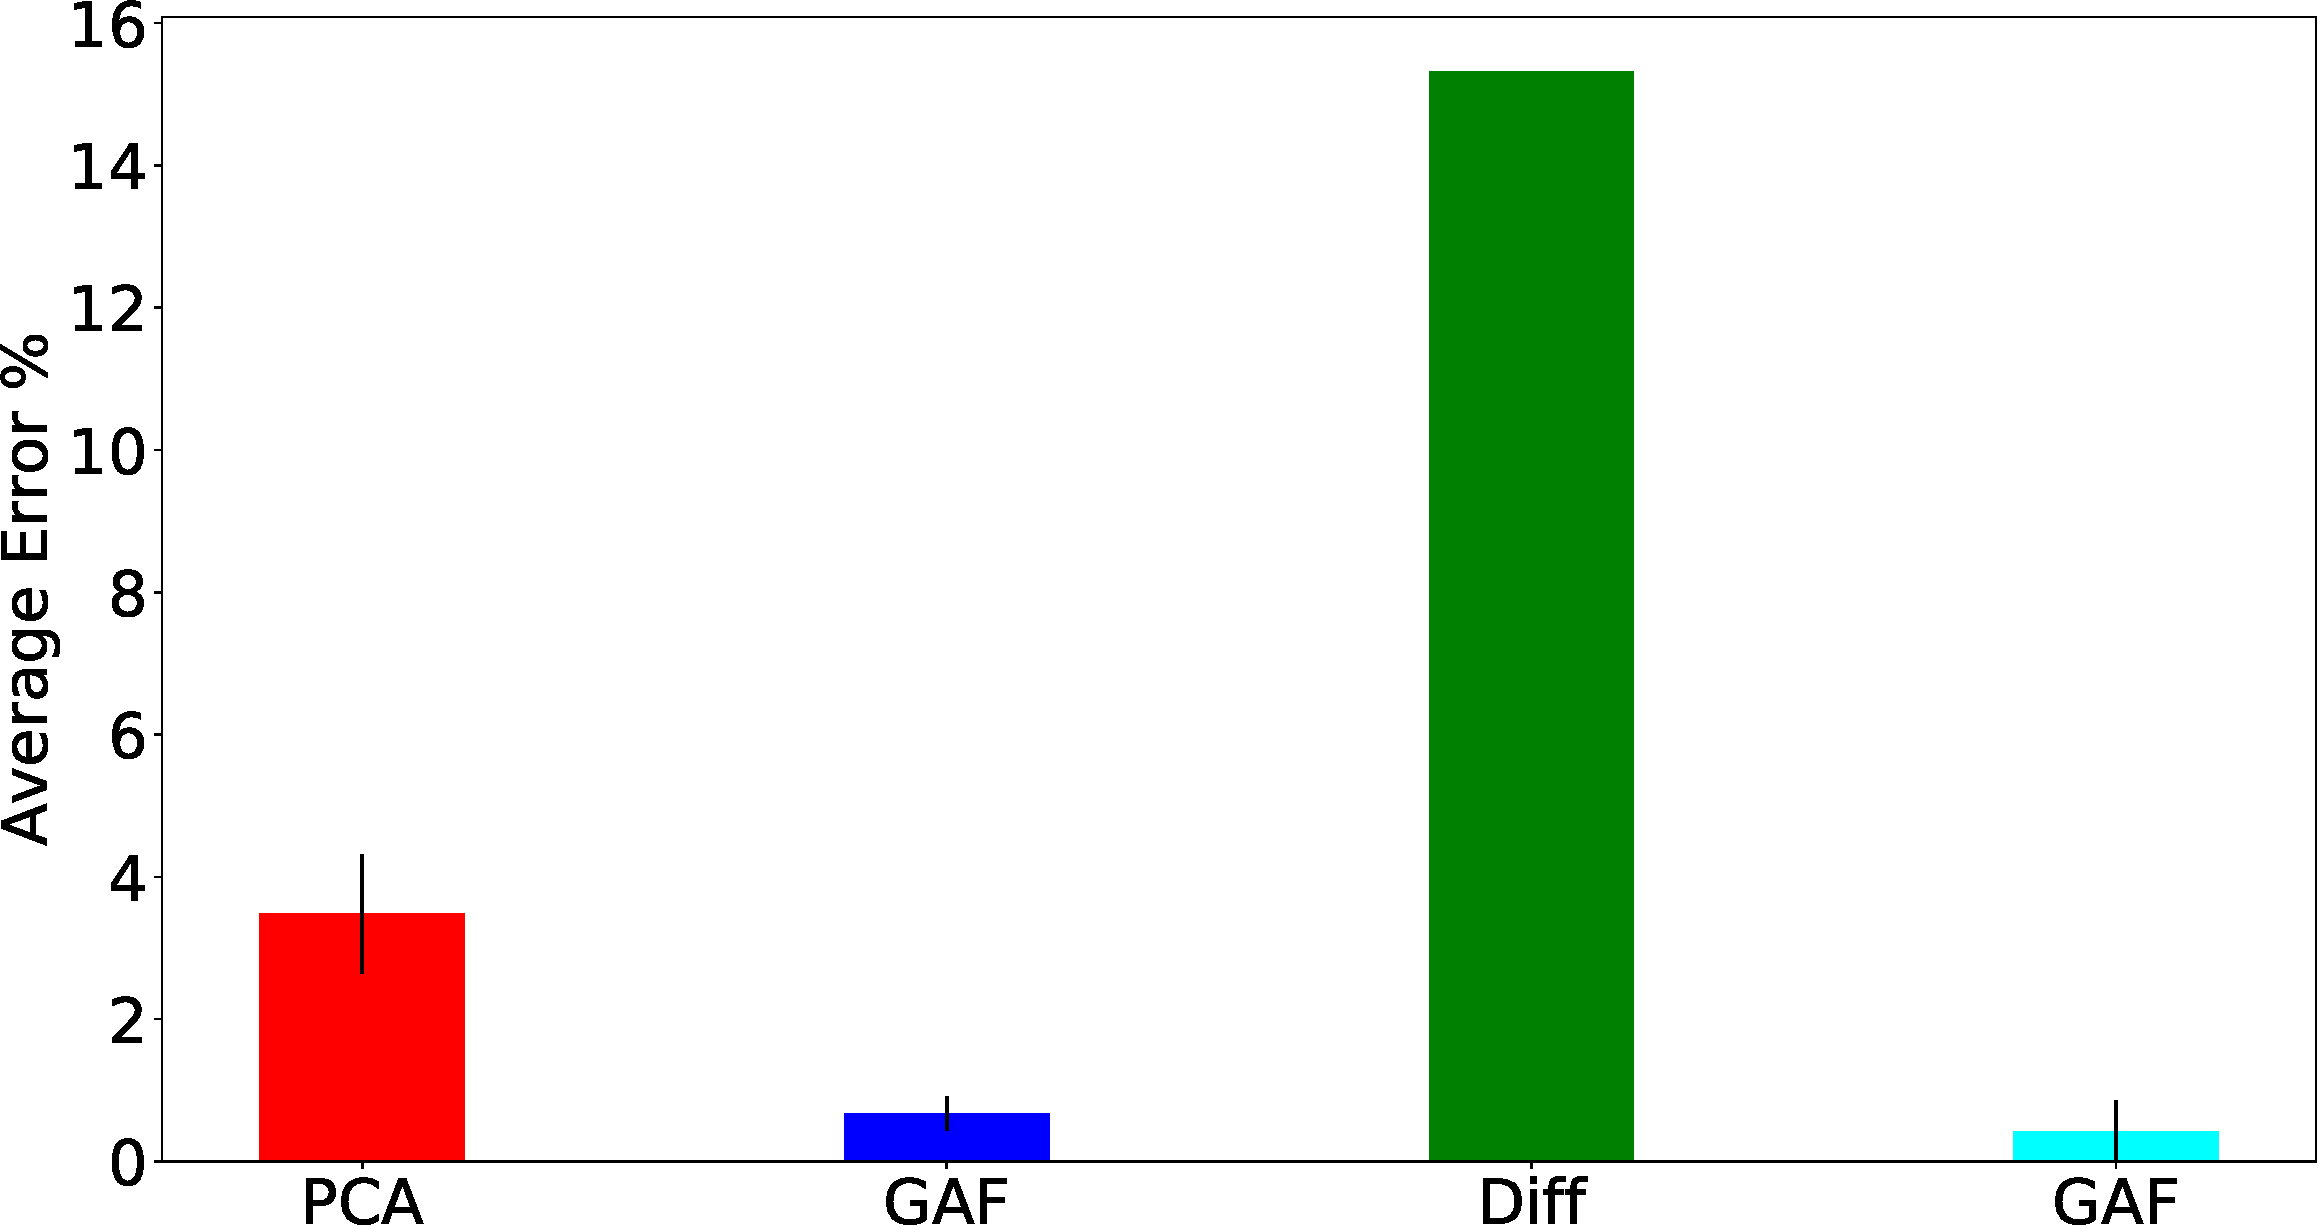
\includegraphics[width=0.48\textwidth]{results-crop.pdf}
 \label{fig:results}
 \caption{The average error for each of the experiments presented in Section~\ref{sec:exp} are presented in this figure. The average error is computed by averaging the diagonal elements of a confusion matrix. The error associated with the computed values are indicated with a black vertical line at the top of each bar.}
\label{fig:results} 
\end{figure}

%Given this background, let us list the  contributions that we make in this paper: 
%\begin{itemize}
% \item Our indepenent study corroborates the study made by Dias et al, i.e. we have confirmed that the GAF transform is a usefull encoding scheme that can be used for pixel-based land cover classification. 
% \item We show that the GAF transform can be utilized for detecting settlement expasion.
% \item We show that the GAF transform can not only be used for pixel based land cover classification, but also for detecting land cover change.
% \item We show that is the classification problem at hand is seperable enough
%\end{itemize}




% Below is an example of how to insert images. Delete the ``\vspace'' line,
% uncomment the preceding line ``\centerline...'' and replace ``imageX.ps''
% with a suitable PostScript file name.
% -------------------------------------------------------------------------


\begin{figure*}[h] 
  \begin{subfigure}[b]{0.5\linewidth}
    \centering
    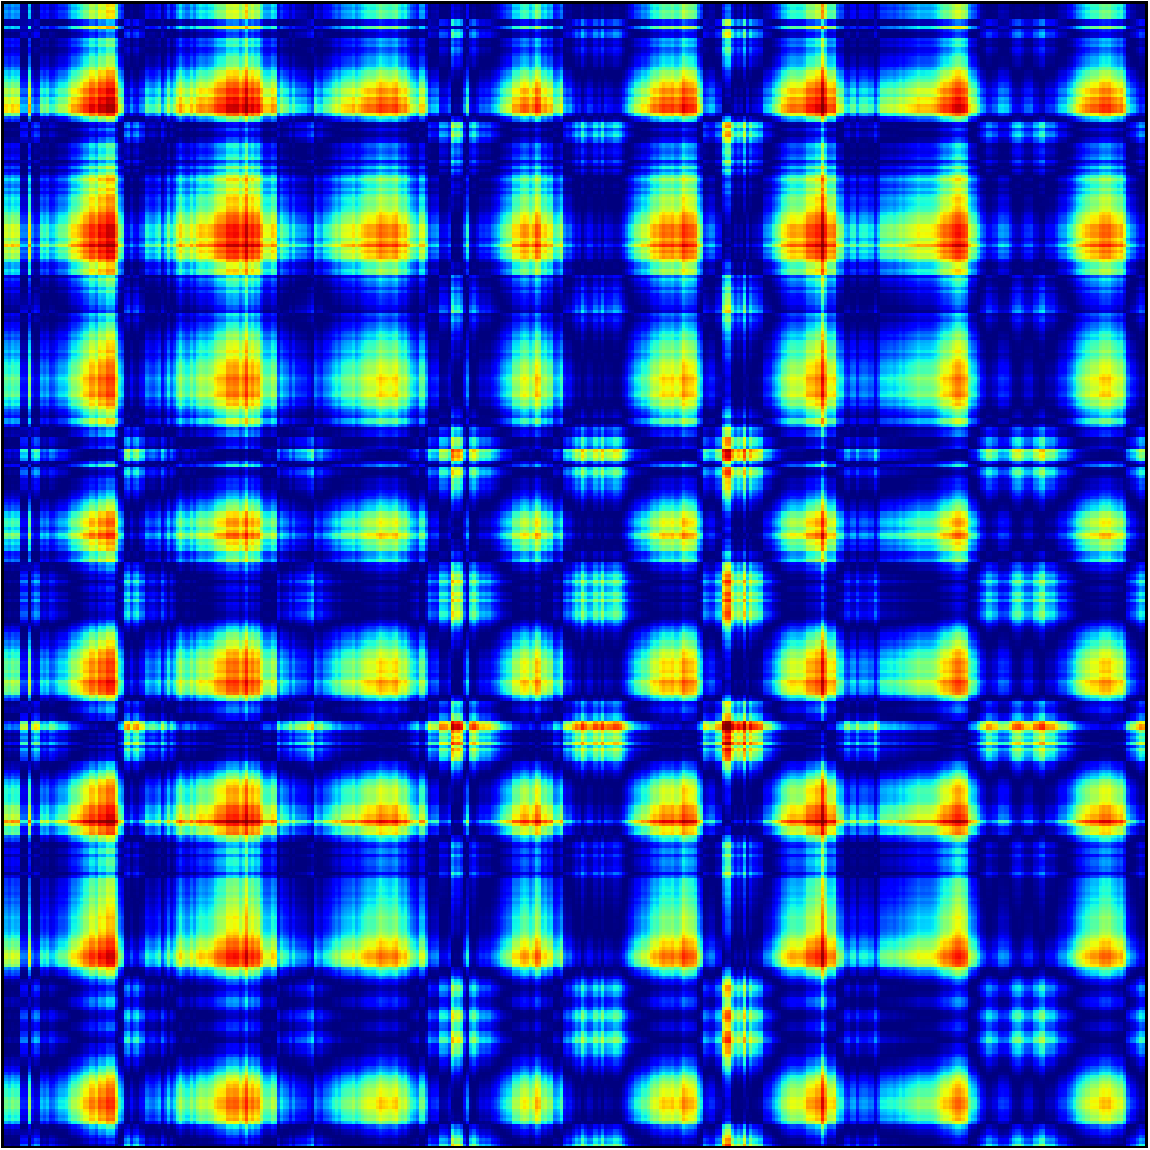
\includegraphics[width=0.89\linewidth]{veg-crop.pdf} 
    \caption{Vegetation} 
    \label{fig7:a} 
    \vspace{6ex}
  \end{subfigure}%% 
  \begin{subfigure}[b]{0.5\linewidth}
    \centering
    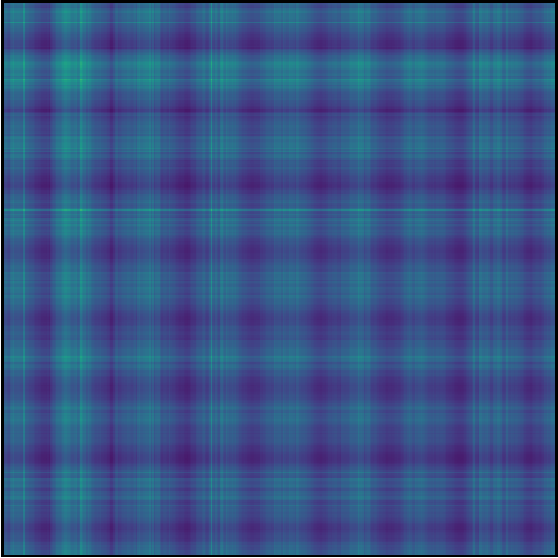
\includegraphics[width=0.89\textwidth]{bwt-crop.pdf} 
    \caption{Settlement} 
    \label{fig7:b} 
    \vspace{6ex}
    \end{subfigure} 
    %\vspace{13ex}
  \begin{subfigure}[b]{0.5\linewidth}
    \centering
    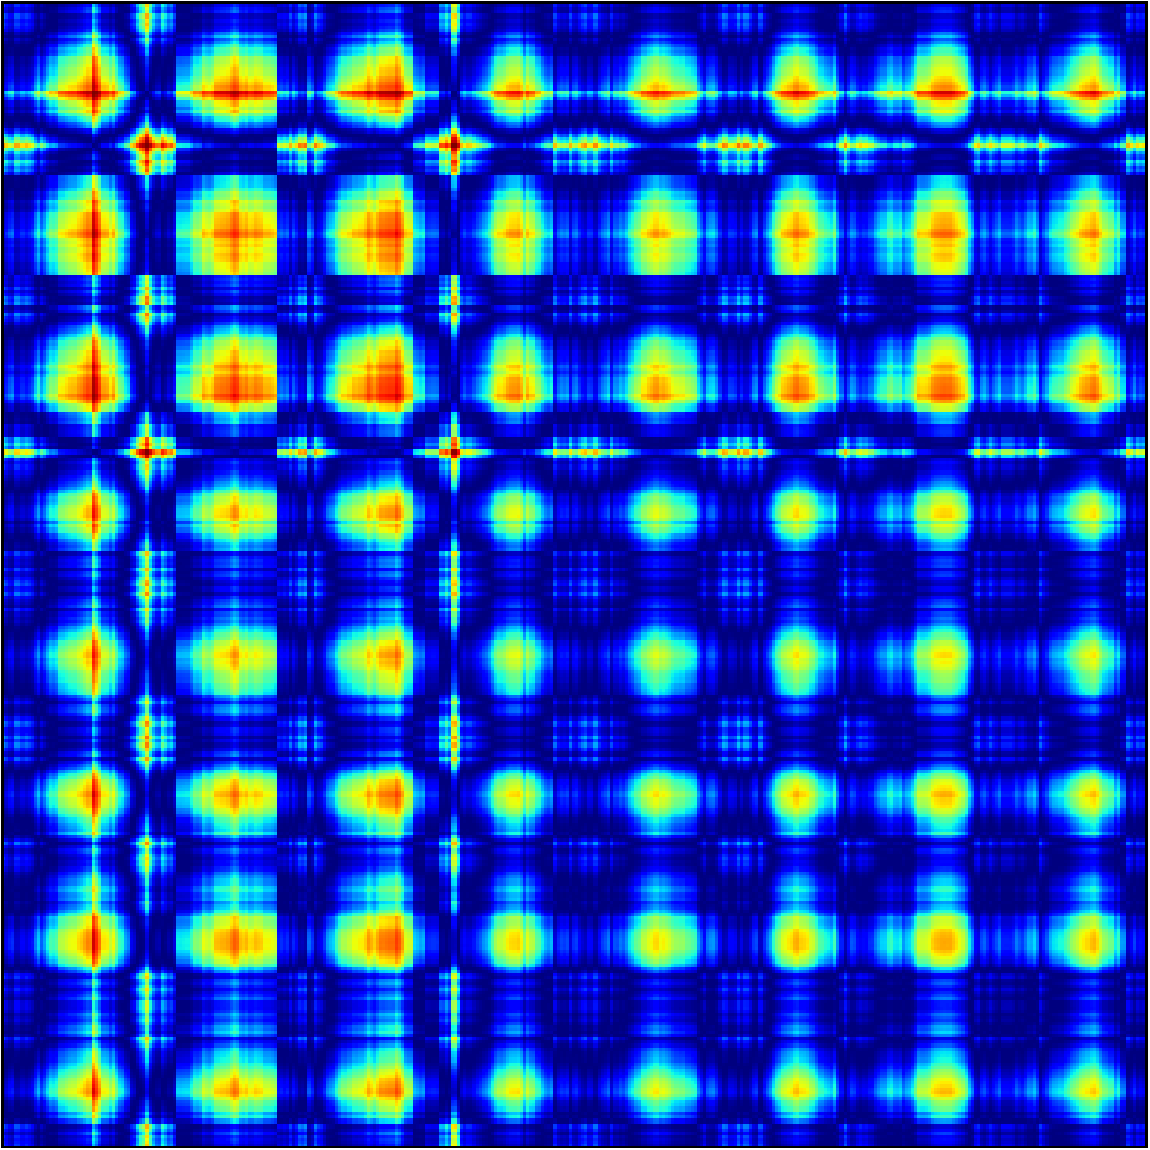
\includegraphics[width=0.89\textwidth]{sim_c-crop.pdf} 
    \caption{Simulated Change} 
    \label{fig7:c} 
  \end{subfigure}%%
  \begin{subfigure}[b]{0.5\linewidth}
    \centering
    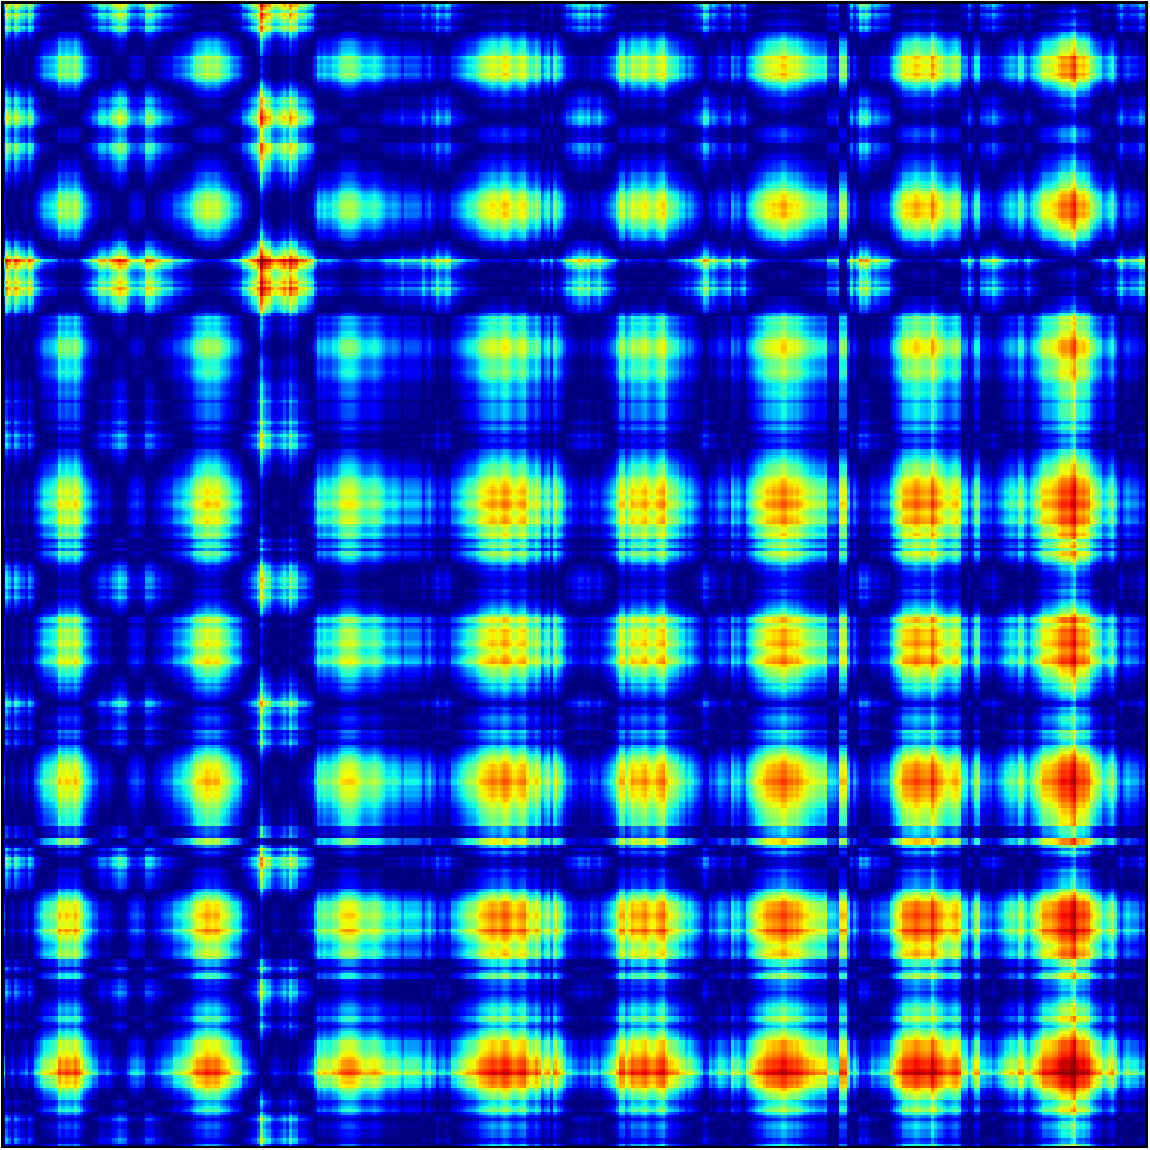
\includegraphics[width=0.89\textwidth]{real_c-crop.pdf} 
    \caption{Real Change} 
    \label{fig7:d} 
  \end{subfigure} 
  \label{fig:gaf}
  \caption{The GAF encoding of a random vegetation pixel (top left), a random settlement pixel (top right), a random synthesized changed pixel (bottom left) and a random real change pixel (bottom right) (see Section~\ref{sec:exp}). The GAF transform encodes time-series as images so that the capability of image-based classifiers can be exploited to perform time-series classification (see Section~\ref{sec:GAF}).  The two images in the top panel are visually discernible from one another. The bottom two images are more irregular in nature than the images in the top panel.}
  \label{fig:gaf}
\end{figure*}






% To start a new column (but not a new page) and help balance the last-page
% column length use \vfill\pagebreak.
% -------------------------------------------------------------------------

%\section{REFERENCES}
%\label{sec:ref}

%List and number all bibliographical references at the end of the paper.  The references can be numbered in alphabetic order or in order of appearance in the document.  When referring to them in the text, type the corresponding reference number in square brackets as shown at the end of this sentence \cite{C2}.

% References should be produced using the bibtex program from suitable
% BiBTeX files (here: strings, refs, manuals). The IEEEbib.bst bibliography
% style file from IEEE produces unsorted bibliography list.
% -------------------------------------------------------------------------
\bibliographystyle{IEEEbib}
\bibliography{strings,refs}

\end{document}
